\newpage
\subsection{Implementation of the embedded server}
\label{sec:embedded_service_impl}
This server can be implemented using any suitable hardware and software.
Chosen tools and libraries are not fixed and can be easily changed in
future.
Loosely coupled modules in the system give a possibility to change everything
without a need of global redesign.

The reason why technologies below are used is that they are simple to use and
easy to learn. They are also quite lightweight and therefore they can be used in
a embedded system.

\subsubsection{Hardware}
\label{sec:hardware}
\begin{center}
 \begin{figure}[h]
	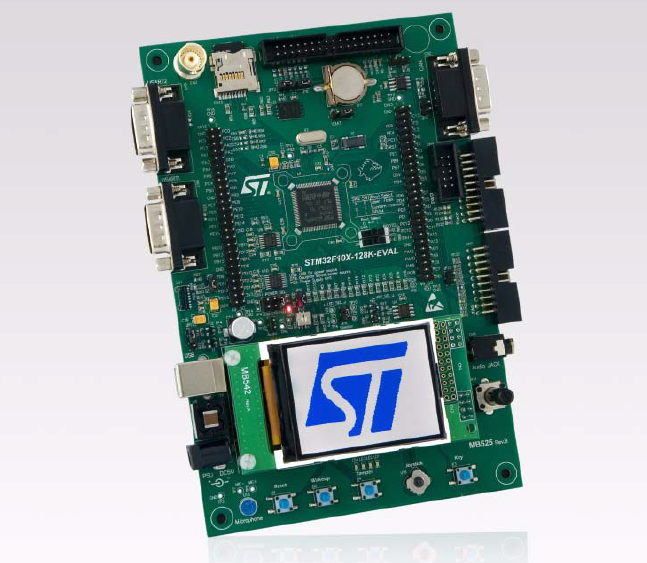
\includegraphics[height=0.5\textheight]{../images/implementation/embedded_server/stm3210b-eval.png}
	\caption{STM32F10X 128K evaluation board (STM3210B-EVAL)
	\cite{stm_eval_board_manual}}
	\label{fig:stm_eval_board}
 \end{figure}
\end{center}

The hardware used in this work are the two ARM Cortex M3 microcontrollers from
STMicroelectronics(\url{http://www.st.com/}). They were chosen because the
company already has a development board  and some other products from that
manufacturer. There is nothing special in that hardware and similar
microcontrollers from other manufacturers may be used in the same way.

The hardware features desribed below are common for almost all microcontrollers
and every well known manufacturer has similar device family.

Description will start from the first used STM32 microcontroller and
the STM3210B-EVAL evaluation board from STMicroelectronics.
These are features that this board has \cite{stm_eval_board_manual}:
\begin{itemize}
  \item Three 5V power supply options: power jack, USB connector or daughter
  board
  \item Boot from user Flash, test Flash or SRAM
  \item Audio play and record
  \item 64Mbyte MicroSD card
  \item Type A and Type B smartcard support
  \item 8Mbyte serial Flash
  \item I2C/SMBus compatible serial interface temperature sensor
  \item Two RS232 communication channels with support for RTS/CTS handshake on
  one channel
  \item IrDA transceiver
  \item USB 2.0 full speed connection
  \item CAN 2.0A/B compliant connection
  \item Induction motor control connector
  \item JTAG, SWD and trace tool support
  \item 240x320 TFT color LCD
  \item Joystick with 4-direction control and selector
  \item Reset, wakeup, tamper and user push buttons
  \item 4 LEDs
  \item RTC with backup battery
  \item Extension connector for daughter board or wrapping board 
\end{itemize}

As you see there are lots of opportunities to apply your creativity.
The amount of features is quite big, but we do not need most of them.
Required are only connectivity(RS232, USB) and debug(JTAG, SWD) interfaces.

This development board is made for evaluation of STM32F10x family
microcontrollers. These are ARM Cortex-M3 core-based mainstream microcontrollers
with a maximum CPU speed of 72 MHz and Flash memory amount from 16 Kbytes
to 1 Mbyte. They are equipped with large variety of peripherals.
\autoref{fig:stm32f103vbt6_hardware} covers interfaces of STM32F103VBT6 MCU that
is used in this board.

This controller is equipped with 20KB SRAM and 128KB Flash memory.
It has three USART transceivers and the debugging interface.
These are the main features we need.

\begin{center}
 \begin{figure}[h]
	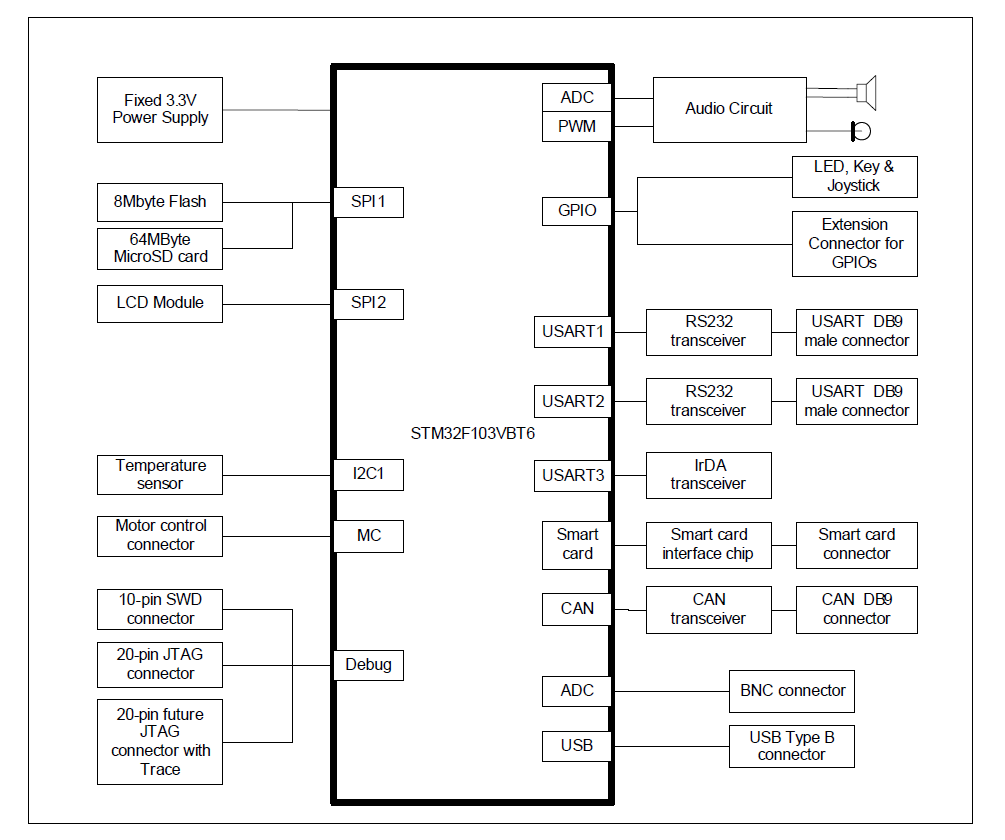
\includegraphics[height=0.5\textheight]{../images/implementation/embedded_server/stm32f103vbt6_hardware.png}
	\caption{Hardware block diagram of STM32F103VBT6 MCU on STM3210B-EVAL board
	\cite{stm_eval_board_manual}}
	\label{fig:stm32f103vbt6_hardware}
 \end{figure}
\end{center}

The second microcontroller that was used  is the STM32F103ZE MCU. It has more
memory:
64KB SRAM and 512KB Flash memory. This controller was chosen because the first
one has not enough resources, especially SRAM memory. The text messages, that
are transferred from client to server and back, require to be stored in the RAM
memory and each request has several copies of data while it is processed.
Amount of RAM on the first MCU was enough to execute optimized and final version of the server, but during development there is need for
storing additional debug information and to try different libraries.
The second reason is that service contracts are stored in the flash memory.
STM32F103VBT6 has 128 Kbytes of flash, however STM32F103ZE has 512 Kbytes.
System becomes more simple when service contract is stored together with
application code and there is no need to introduce another level of complexity (
connecting external storage device and programming connectivity code for
that). 


STM32F103ZE has 5 USART interfaces which is more than enough for this kind of
system. Three of them are used in the application: One for client-server
communication, one for logging and the third one for communicating with coffee
machine.

Client and server are connected using Bluetooth-to-serial module LMX9838 from
Texas Instruments.This module contains hardware and firmware support of
Bluetooth and Serial Port Profile and can be used as simple wireless serial
interface in communication between devices.

Server logging interface is connected to a personal computer using FTDI
Serial-to-USB chip (\url{http://www.ftdichip.com/}). This is popular solution of
connecting embedded systems and USB powered hardware. There is the virtual com
port on the PC side, that is powered by drivers of operating system. This
solution can be used instead of old serial connectors, that are not always
available on modern hardware.

Embedded service server and coffee machine are connected using serial line and
wires. This is a most simple connection here. Coffee machine has external serial
interface and STM32 microcontroller is connected directly to it.

That was a short overview of system hardware. Next comes description of system
software and operating system.

\subsubsection{Software and operating system}

\paragraph{Hardware configuration} ~\\
All MCU hardware is controlled by the software.
The execution of a trivial program (like "Hello world") on a
microcontroller requires a long list of instructions. To write some bytes to
UART or to blink with LED you usually need to:
\begin{enumerate}
  \item Configure MCU clock. Select clock source, frequency, clock prescalers
  \item Configure clock for peripheral buses. Again, the source and frequency by
  configuring prescalers. (Advanced Peripheral Bus in case of ARM)
  \item Turn on clocking for buses and peripherals.
  \item Configure general purpose input/output (GPIO) ports to use required
  function.
  \item Configure interrupt controller for the peripherals.
  \item In case of UART or any other communication, set the communication speed
  and configure the interface parameters.
  \item Write your application code
  \item Download the code to the device
  \item Debug the results
  \item Start from the beginning.
\end{enumerate}

Modern MCUs, especially with ARM Cortex-M architecture, have very complex
structure. They contain a huge amount of interfaces ( see \ref{sec:hardware}
section and feature list of evaluation board ) in a one single chip.
Most of peripherals are separately clocked, which gives a possibility to turn
off inactive ones and save the power energy. During MCU system startup
programmers code  should turn on and configure required peripheral modules.

In contrast, traditional software developing for desktop computers requires only
last four steps and the most complicated preparation step is the compiler and
IDE environment setup.

Each "configuring" step requires deep knowledge about what you are doing. MCU is
configured by values that are stored in memory mapped control registers. Each
register has a special purpose and different values written there configure
various MCU modules. In general words, you need to know these values to
configure the MCU system properly. Each bit in the control register represent
some setup setting.

Every controller family from various manufacturers differs from each other.
Therefore there is no need to write here in deep details how to configure one
special MCU named STM32F103ZE from STM32F1, what values to write into
\texttt{USART1->CR1} control register and which register bit turns on the UART
parity check. These instructions are not portable. When MCU hardware
changes(even families from a single manufacturer may highly differ) you need to
write this part once more.

There are two possible and more portable ways how to configure a STM32
microcontroller: Using CMSIS\footnote{The ARM® Cortex™ Microcontroller Software
Interface Standard (CMSIS) is a vendor-independent hardware abstraction layer for the Cortex-M processor series.}
from ARM and Standard Peripheral Library from STMicroelectronics. These are
hardware abstraction layer libraries that help to write portable code. They
define standard  application programming interface (API) for the ARM
architecture. Hardware vendors provide CMSIS compliant bindings for their
hardware and programmers may write their code in standard manner, reducing
resources for platform change and reusing existing code.

Standard Peripheral Library is a C language library that provides standard API
for programming STM microcontrollers. It also contains CMSIS inside for
managing ARM core. There are several data structures, macros and functions that
help to configure and manage MCU peripherals.
The famous UART may be configured using Standard Peripheral Library like this:

\begin{listing}[H]
\begin{minted}[frame=lines,
               framesep=2mm]{c++}
RCC_APB2PeriphClockCmd(RCC_APB2Periph_USART1, ENABLE);

USART_InitTypeDef USART_InitStructure;
USART_InitStructure.USART_BaudRate = 115200;
USART_InitStructure.USART_WordLength = USART_WordLength_8b;
USART_InitStructure.USART_StopBits = USART_StopBits_1;
USART_InitStructure.USART_Parity = USART_Parity_No;
USART_InitStructure.USART_HardwareFlowControl = USART_HardwareFlowControl_None;
USART_InitStructure.USART_Mode = USART_Mode_Rx | USART_Mode_Tx;
USART_Init(USART1, &USART_InitStructure);
\end{minted}
\caption{USART1 initialization using Standard Peripheral Library}
\label{lst:uart_init_example}
\end{listing} 

Most of configuration can be done using preprocessor defines.
You may add several defines, for example \texttt{\#define STM32F10X\_MD} to use
STM32 Medium density devices (Flash memory density ranges between 64 and 128
Kbytes). Clock rates and different peripherals can be adjusted in a similar way.

The distribution of STM Standard Peripheral Library contains a lot of
code and application examples, that helped me a lot. I have found there how to
configure a USART DMA\footnote{Direct Memory Access} controller and how to
transfer bytes using USART without intervention of central processing unit.
This is  quite good source for the beginners like me.

Setup an embedded development environment takes a lot of time and requires
deep knowledge about the underlying hardware. It is good to have such tools like
standard APIs, that help to make this process more easy.

\paragraph{Operating system} ~\\
Programs for embedded devices can be written in many different ways.
Some traditional ways how to do it:
\begin{itemize}
\item One big while loop and polling resources(also called busy waiting)
\item The same while loop, but it is interrupt driven.
Interrupts change some global variables inside interrupt service routine (ISR)
and main loop checks them on the next program cycle
\item The use of multitasking realtime operating system (RTOS) 
\end{itemize} 

The two first methods are often called bare metal approach.
Bare metal refers to techniques where programmers directly control and manipulate the underlying core, performing register-level access setting and clearing bits, and moving and operating on bytes of data directly.
Everything traces directly to the programmer’s next line of code being executed, and there is nothing in between the programmer and the hardware.
Resources like timers, interrupts, and I/O have to be accounted for in the application code.
The bare metal approach works well when a system has a  well defined and deterministic processing algorithm, only a couple of tasks to manage, or needs precise instruction level determinism(hard realtime).

Operating systems for microcontrollers have features like: 
multitasking/multithreading,task prioritization, interprocess communication, memory management, abstracted I/O drivers, file systems, networking.
They give to programmer higher level of abstraction and standard APIs, which help to reuse already existing code.
Popular RTOS already come with various protocol stack and drivers implementations.
However, the greatest feature they have is the multitasking. 
The program could be divided into several separate tasks and these tasks could run in the parallel.
Parallel execution is achieved by dividing available CPU time between tasks.
This process is called \textit{scheduling}. 
There are two main scheduling policies: cooperative scheduling and preemptive scheduling.


During cooperative scheduling CPU time is used by a task until this task explicitly gives CPU time to other tasks.
This means that if the task will not give this time to others the whole system will hang.
This approach gives reliable and deterministic control over all tasks  and programmer needs to define CPU time release points.
There is no need of protection of common resources, because each task controls its execution and another task could run in that moment.

The second preemptive scheduling approach gives each task a regular "slice" of operating time. 
Each task has defined amount of CPU time during which it is able to do useful work.
Scheduler takes this time when this time is over and gives this to another task.
These tasks could have priorities, which allows to execute essential tasks before the background are executed.
At the moment of the task context switch scheduled decides which task will be next according to the priority of available tasks.
Task with a higher priority will be triggered next. 
Scheduler should also be able to give the execution time to tasks with lower priorities, otherwise the will be never triggered because tasks with higher priorities will be launched instead.
Tasks with the same priorities are executed one by one in the loop~\cite{barry2010using}.
Such scheduling algorithm gives the illusion that tasks are running in parallel.
Parallel task execution requires protection of common and global hardware resources. 
For example, the situation when some task can change a global variable, while another task is reading it and makes some decision.
The result is that second task receives invalid result, which was modified between assigning a check value to some variable and reading it.


The coffee machine service application contains many different task like: 
multiple communication handling,
request processing,
request deserialization, etc.
This amount of tasks is not final.
This system needs to be extensible.
There should be an opportunity to add new request and communication handlers.
Request processing by the server is the concurrent process: while several requests are processed, another requests are sent over the network and communication interface needs to receive them.
Response transmitting could also run in parallel.

It becomes harder to maintain and develop such concurrent program if you are not using a multitasking system. 
You need always to carefully think where to insert a functionality into a big polling loop.
Each insertion requires reordering of control statements and checking the execution order of all parallel tasks.
Moreover, your application may handle two different independent tasks and you need to keep data separated and remember which task does each variable belong.
The use of operating system helps to keep things separated and loosely coupled.
 
\paragraph{FreeRTOS} ~\\
FreeRTOS is a popular real-time operating system for embedded devices, which has
ports for many MCU devices(34 architectures \cite{FreeRTOS_website}),
also including STM32F1 family microcontrollers.
This operating system was chosen for the embedded service application implementation in this work.
The reason is that this operating system has low entry level for the beginners and good documentation.
In addition to that i have found and read a book \cite{barry2010using}, which is a great introduction to FreeRTOS and embedded multitask systems programming. 

FreeRTOS has several features described below~\cite{FreeRTOS_website}:
\begin{itemize}
\item Pre-emptive scheduling option 
\item Co-operative scheduling option
\item ROMable
\item 6K to 10K ROM footprint
\item Configurable / scalable
\item Compiler agnostic
\item Some ports never completely disable interrupts
\item Easy to use message passing
\item Round robin with time slicing
\item Mutexes with priority inheritance
\item Recursive mutexes
\item Binary and counting semaphores
\item Very efficient software timers
\item Easy to use API 
\end{itemize}

All this features and support of available hardware helped to make a choice of using FreeRTOS in this project.
I was inspired by this easy to use API, spread documentation and verbose examples.
Next i will describe some essential FreeRTOS APIs  and how tasks are created and managed.

The next thing you need to make after the setup of the programming environment and writing a trivial program to test it is the definition of system tasks.
A task in FreeRTOS is usual C function and
listing \ref{lst:freertos_task_function_prototype} contains a prototype of this
function.


\begin{listing}[H]
\begin{minted}[frame=lines,
               framesep=2mm]{c++}
void ATaskFunction( void *pvParameters );
\end{minted}
\caption{FreeRTOS task function prototype}
\label{lst:freertos_task_function_prototype}
\end{listing} 

Implementation of this function usually contains a separate program which has  infinite loop and never exits.  
Creation of temporary tasks which are finite is also possible.
Tasks may be deleted in the runtime using \texttt{vTaskDelete()} function.
Task function has no return type (void) and \texttt{return} statements are not allowed, they should be explicitly deleted.
It accepts method parameters of void pointer type, which allows to pass any type parameter there.
Required parameter needs to be casted to \texttt{void*} before passing the parameter.
It can be used inside task function through casting back to original type. 
This feature is used to pass a complex configuration structure to a system task in the embedded service design.

Task function do some useful application work. In order to start they require a registration in a system scheduler.
When microcontroller program first starts, it gets into reset interrupt service routine, where starts the hardware initialization process.
The \texttt{main()} application method is called after all hardware is initialized.
All tasks should be started in that \texttt{main()} application method, where the first application code usually starts.
Listing \autoref{lst:freertos_task_create_function_prototype} shows task
creation function prototype.
\begin{listing}[H]
\begin{minted}[frame=lines,
               framesep=2mm]{c++}
portBASE_TYPE xTaskCreate( 
	pdTASK_CODE pvTaskCode, 
	const signed portCHAR * const pcName, 
	unsigned portSHORT usStackDepth, 
	void *pvParameters, 
	unsigned portBASE_TYPE uxPriority, 
	xTaskHandle *pxCreatedTask 
);
\end{minted}
\caption{FreeRTOS task function prototype}
\label{lst:freertos_task_create_function_prototype}
\end{listing} 

The first parameter is the pointer to a task function, which has the application logic.
Second parameter is the name of that task. It is used for system needs like debuging.
Parameter with name \texttt{usStackDepth} configures available stack space for the task.
Each context switch and method calls in a task use that memory space for storing application context.
Program counter and state of the operation registers are stored there.
All local variables are also copied to the stack during context switch.
Therefore this parameter should depend on the complexity of the application (function call depth) and
amount of local variables used in each child function. 
The fourth parameter is a pointer to the task parameters. Next parameter defines priority of that task.
The last one is the pointer to the task handle structure, which should be defined before this method call.
\texttt{xTaskCreate()} method returns a handle.  This handle may be used to
control  this task.

This method only creates  tasks, but not executes. 
\texttt{main()} application method should contain a \texttt{vTaskStartScheduler()} call, that executes the scheduler and registered tasks are executed by this scheduler.
\texttt{vTaskStartScheduler()} call is normally a blocking call, it never ends and runs until there is some error.
On error scheduler method finishes and program execution returns to the
\texttt{main()} application method, where program continues to run.


Task can force a contex switch by calling \texttt{taskYIELD()} method.
FreeRTOS scheduling algorithm  can be configured as cooperative or preemptive.
In cooperative scheduling mode \texttt{taskYIELD()} method is used to make a
context switch and give CPU time other tasks.
In preemptive it forces a context switch before time slice has ended.
Another task can start from the middle of the time slice of previous task.
This gives better overall system performance.

FreeRTOS uses queues for interprocess communication.
Queues can be used to send messages between tasks, and between interrupts and
tasks. 
In most cases they are used as thread safe FIFO (First In First Out) buffers with new data being sent to the back of the queue, although data can also be sent to the front. 

The queue operations are  mutually exclusive ( see listing
\autoref{lst:freertos_queue_methods}).
The same queue element cannot be received twice in different tasks.
Messages are sent through queues by copy, creation of the queue allocated memory
space and queue insert function copies inserted value to that space.
You hold different values in a queue: this may be plain C language primitive
type, a structure or even \texttt{void*} type. Large structures can be sent by
storing a structure reference pointer. 
Queue functions are also blocking functions. Delay amount measured in system
ticks can be provided to queue functions, it is able to lock forever by passing
a special system value to these functions. Operation methods also return status
of the operation.
 

\begin{listing}[H]
\begin{minted}[frame=lines,
               framesep=2mm]{c++}
xQueueHandle xQueueCreate( 
	unsigned portBASE_TYPE uxQueueLength, 
	unsigned portBASE_TYPE uxItemSize 
); 

portBASE_TYPE xQueueSendToFront( 
	xQueueHandle xQueue, 
	const void * pvItemToQueue, 
	portTickType xTicksToWait 
);

portBASE_TYPE xQueueSendToBack( xQueueHandle xQueue, 
	const void * pvItemToQueue, 
	portTickType xTicksToWait 
); 

portBASE_TYPE xQueueReceive( 
	xQueueHandle xQueue,
	const void * pvBuffer, 
	portTickType xTicksToWait 
);

portBASE_TYPE xQueuePeek( 
	xQueueHandle xQueue,
	const void * pvBuffer, 
	portTickType xTicksToWait 
);
\end{minted}
\caption{FreeRTOS queue methods}
\label{lst:freertos_queue_methods}
\end{listing} 

\begin{center}
 \begin{figure}[H]
	\centering
	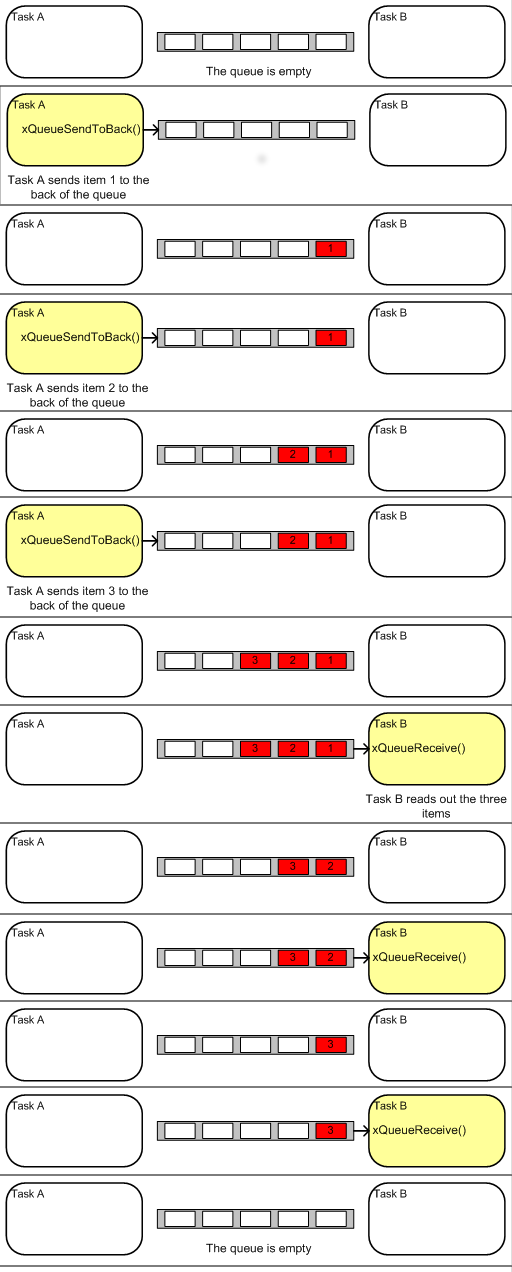
\includegraphics[height=\textheight]{../images/implementation/embedded_server/queue_ipc.png}
	\caption{Writing to and reading from a queue.\cite{FreeRTOS_website}}
	\label{fig:queue_ipc}
 \end{figure}
\end{center}

Semaphores and mutexes are based on the queues and their methods are similar to
queue methods.
They can protect your sensitive data from being changed from other tasks.
\texttt{xSemaphoreTake()} and \texttt{xSemaphoreGive()} are used for that
purpose. There are also available mechanism of critical sections.

FreeRTOS has own memory management mechanism and there are four memory
allocation  options available:
\begin{enumerate}
  \item Memory can be allocated, but it cannot be freed. This option is for
  static applications, which allocate memory only at system startup and use that for
  the lifetime of program 
  \item  Best fit algorithm is used. Memory can be freed. This approach does not
  combine free blocks into a single large block and memory gets fragmented. This
  is not good for applications who allocate random memory size.
  \item  In this option the standard C library \texttt{malloc()} and
  \texttt{free()} functions are used. This is a standard way of memory
  allocation and it is supported by the compiler and linker.
  \item This scheme uses a first fit algorithm and, unlike scheme 2, does
  combine free memory blocks into a single large block
\end{enumerate}

Options other than 3 are more efficient than standard \texttt{malloc()}
and \texttt{free()} and are thread safe. Their footprint is smaller and work in
pair with the OS kernel. 

I tried several options and ended up with the last configuration option. 
Option 3 was not stable for me and system frequently crashed while using it.
Therefore last approach was chosen as more stable. Memory heap is stored inside
one big byte array and memory allocator takes a free space from there.

FreeRTOS may be used in various applications and it contains lots of useful
functionality. It can be extended using different modules ( see
\cite{FreeRTOS_website}) like networking modules (TCP and UDP), input output
modules, filesystem modules and others. It is a quite good choice for a newbie
like me. There is no need to reinvent the wheel.

\subsubsection{Service software}


Previous section was mainly about available features in the operating system and
hardware. 
This section covers how the software of embedded server is written
using some of them.

\paragraph{Initialization} ~\\
Application starts with hardware initialization code. Microcontroller clock
source is external quartz oscillator (8 Mhz) and MCU is configured to use 
PLL(Phase locked Loop) frequency multiplier,  which is used for multiplying its
input frequency by a given factor of two to sixteen. 
Using the PLL, you can generate clocks up to 72MHz.

Next comes initialization of USART communication interfaces. USART are configured
to use \gls{DMA} controller. \gls{DMA} works in both directions: receive and
transmit. The usage of DMA requires initialization of DMA controller, assigning
destination/transmitting memory buffer and buffer length, and other configuration
parameters. DMA may be configured to use memory increment and data direction (
from the peripheral to buffer or from buffer to peripheral). This feature
enables sending and receiving data to/from the USART without utilization of
CPU.

In case of transmitting the data, program may store data to the memory
buffer, trigger DMA send event and continue further processing. DMA controller
sends the data bytes to USART one by one until incremented memory address is
equal to the length of the buffer. Interrupt is generated after operation
completion (or in case of error, you need to check status flags to extract
operation status), which signalizes end of transmission operation to user.
While DMA is sending data, CPU can prepare next bulk of data to send.

Receiving of data works in a similar way.
Three types of DMA interrupts are used for that:
\begin{itemize}
  \item DMA Full transfer interrupt indicates that full buffer transfer was
  ended
  \item DMA Half transfer interrupt routine triggers when the half of the
  transmitting buffer is sent
  \item USART idle interrupt indicates that the
  line is free and there are no more characters.
\end{itemize}  
When the DMA half interrupt occurs user receives first half of the receive
buffer. Second half of the buffer may be taken by the user after the full
transfer interrupt. Line idle interrupt service routine is triggered when the
line is free for some amount of time. Programmer needs to check what is the
current status of the transfer and how many bytes are already received by the
DMA controller. Current position( first half or second half of the buffer) can
be calculated according that value and the right chunk of bytes can be
extracted.

Interrupt service routines store incoming bytes in a FIFO(First In First Out)
buffer. Application note \cite{stm_dma_fifo_appnote} contains description of
this approach. In short, two receive buffers are used: one for DMA controller
and another is for user application. There are some problems using traditional
one buffer implementation: user software should retrieve data from the
receive buffer before the data are overwritten by the next received data.
Receive buffers are often implemented in a circular way( DMA also has this
option) and when buffer is filled, write pointer returns to the start of the
buffer and data may be written again. User needs to read this data or it will be
overwritten. In a double-receive-buffer approach the second buffer, which
belongs to the user, is not overwritten. The code implemented by me just ignores
to write into user buffer when it is full. There is a tradeoff while user is
inactive and does not read anything: 
to loose all the data and overwrite all buffer with new bytes or to loose only
some part of it. That is how receiving of the message works in the embedded
server described in this work.

After initialization of the USART transceivers and their DMA, program initializes 
FreeRTOS tasks and data structures. All system queues and semaphores are created
at that time. Tasks are registered and task input parameters are passed into
task functions. Next scheduler is started and all tasks start to run. Scheduler
works forever while system is powered.

This is how successful scenario looks like. There are also another ones:
\begin{itemize}
  \item There is unable to create tasks and data structures (not enough memory
  or some error)
  \item There is not enough memory to start all tasks and scheduler function
  exits and program crashes.
  \item A stack of some task gets overflowed and task crashes.
  \item There is not enough memory in a heap and task cannot allocate memory
  for new objects. As a result program crashes.
\end{itemize}

All this events are signalized by the FreeRTOS kernel and programmer needs to
decide what to do if some of them happens. Our application is in early stage
development and error conditions are handled using unlimited loops.
Program gets into this loop and it is able to watch stack trace in the debugger
and find a place where it was behaved incorrectly.

\paragraph{System tasks and their functions} ~\\

The architecture of this embedded server consists of several components.
\autoref{fig:server_components_and_data_flow} shows how they all are connected
together.

\begin{center}
 \begin{figure}[h]
	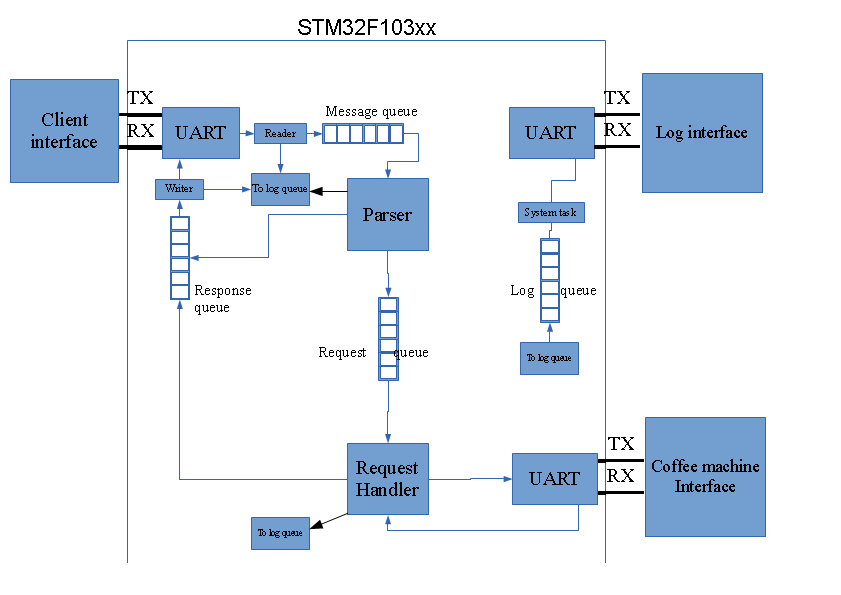
\includegraphics[width=\textwidth]{../images/implementation/embedded_server/system_tasks_and_data_flow.png}
	\caption{System tasks architecture and  the data flow}
	\label{fig:server_components_and_data_flow}
 \end{figure}
\end{center}

Most tasks have similar structure and may be covered with a few lines of code:


\begin{listing}[H]
\begin{minted}[frame=lines,
               framesep=2mm]{c++}
void tskSomeTask(void *pvParameters) {
	while(1) {
		if(uxQueueMessagesWaiting(someQueue) > 0) {
			xStatus = xQueueReceive( 
				systemMsgQueue, 
				&sysMsg, 
				QUEUE_RECEIVE_WAIT_TIMEOUT 
			);
			
			/* 
				make some useful work here
			*/
		}
		vTaskDelay(250 / portTICK_RATE_MS);
	}
}
\end{minted}
\caption{General task function structure}
\label{lst:task_function_structure}
\end{listing}

As it was written before, FreeRTOS tasks are made like unlimited loops.
Usually tasks are waiting for some messages in a queue.
When a message is inserted from somewhere task receives it from the queue and
starts processing. When the work gets done,  task sleeps for define amount of
time. 

Most of task in this system are made using this method. 
Tasks wait for resources and process them. 
They are in sleep most of time.

Task with a higher priority is the task called  \texttt{tskSystem}.
It is started before all other tasks and is responsible of handling system
messages. 
\texttt{tskSystem} is used to output debug information and logging messages.
It is waiting for the message with type \texttt{MSG\_TYPE\_LOGGING} and sends it
over logging UART.
This task wakes between every 250 ms intervals and checks for new logging
messages. It also reports the remaining heap memory size.

Logging messages are sent to a system queue from other tasks.
Logging gives the ability to trace essential processing steps and to quickly
find the broken place.
I have implemented logging API which is similar to Apache log4j in Java
programming language( see \url{http://logging.apache.org/log4j/1.2/} and search
for \textit{log4j} and \textit{slf4j} keywords.
In order to write log message you need to call \texttt{logger(LEVEL\_INFO,
"log message text")} method specifying a level of severity for a message and
message text. There are  lots of these calls in application code. It is
necessary to log all essential moments of application lifecycle. Level with
lowest severity \texttt{LEVEL\_TRACE} may be used for tracking separate method
calls. Each method may have trace logging call at entry and return points.
User can turn of these messages by setting global logging system level to more
higher one (the highest is \texttt{LEVEL\_OFF}).

Other tasks will be covered according to data flow showed in
\autoref{fig:server_components_and_data_flow}.

The first task that meets request from the client is the UART reader task.
At the early state of development this was a special and dedicated task for
reading from one communicating port. Later i changed it to be more common and
function was renamed to \texttt{tskAbstractReader()}. Now this can be a
reader for any source. It is configurable by task input configuration parameters
which have structure showed in listing \ref{lst:reader_config_structure}

\begin{listing}[H]
\begin{minted}[frame=lines,
               framesep=2mm]{c++}
typedef struct _reader_params_t {
	transport_type_t				transport_type;
	stream_read_char_function_t		read_char_func;
	stream_has_byte_function_t		stream_has_byte;
	xQueueHandle					dataInputQueue;
	portTickType					dataInputQueueTimeout;
	xSemaphoreHandle				dataReadSemaphore;
} reader_params_t;
\end{minted}
\caption{Reader configuration structure}
\label{lst:reader_config_structure}
\end{listing}

This task become an abstract because it has common processing algorithm ( which
is similar to algorithm in listing \ref{lst:task_function_structure}).
It waits for \texttt{dataReadSemaphore} in a loop. 
This semaphore is released in DMA \gls{ISR} when UART message arrives.
\texttt{stream\_has\_byte\_function\_t} is a function that returns true
when UART incoming message FIFO has bytes to read. 
\texttt{stream\_read\_byte\_function\_t} returns one byte from the buffer
\footnote{Most programming language have a concept named \textit{streams} or
\textit{data input output streams}. The tutorial located at
\url{http://docs.oracle.com/javase/tutorial/essential/io/streams.html}
(accessed 13-August-2013) introduces this abstraction.}.

This byte can be processed using any algorithm. This is a place where you need
to define a protocol that your application will use.
There are available million and one more communication protocols and this work
covered some of them below. 
This level requires an analogue to  Data link
layer protocols from ISO OSI communication model 
( an example can be Ethernet, Point-to-Point Protocol (PPP), High-Level Data
Link Control (HDLC)  and others). 
Their purpose is to provide an defined
mechanism how pieces of data bytes compose communication frames or packets. 
Frame is a digital data transmission unit in computer networking and
telecommunication. These protocols define which data bytes are control
information and which represent data to be sent.

There should be special byte sequences (or single bytes) which indicate the 
beginning and the end of each communication message. 
The first control symbol i started to use was ASCII newline symbol ('\\n').
Incoming sequences of bytes were separated by a byte with value \texttt{0x0A}.
The messages were line oriented and each incoming line was a new message.

There is a problem using such control mechanism. If your message contains a 
newline( which is very predictable if you are working with text) you receive an
incomplete message and there is impossible to find if received message is wrong
or not. Message gets splitted into two message packets.

I started to improve this solution and the next step was usage of ASCII control
characters like EOT(end of transmission, value \texttt{0x04}), ETB (end of
transmission block, value \texttt{0x17}) and similar. Using these  control
characters you can detect messages in incoming stream, but this does not help in case of transferring data
bytes, which can be any value between \texttt{0x00} and \texttt{0xFF}.


I started a research of suitable protocols that have a solution for that problem.
My mistake was that i started from wrong direction.
I started to read
specification for Point-to-Point Protocol and other Internet related
technologies.
My thoughts were about realization of a complex data packet structure, with lots
of packet members and a complex data flow control in there, like it is in these
technologies. My friends, who are programmers, advised me to create a custom
protocol using \texttt{\mbox{start\_byte:length:checksum:data:end\_byte}} message
structure. This might be that exact structure, but finally i found a solution
from the beginning of my master thesis research - the
website\footnote{\url{http://www.simple-is-better.org/}} of Roland Koebler, which is named \textit{"Simpler is better"}.
The title page of this site contains a beautiful quote:
\begin{quotation} 
Technology always develops from the primitive, via the complicated, to the
simple. \newline
— Antoine de Saint-Exupéry
\end{quotation}

I have found there a very simple solution how to transfer data packets. It is
called \textit{netstrings} ( \url{http://cr.yp.to/proto/netstrings.txt} is the
source specification, last accessed at 13-August-2013). 
A netstring is a self-delimiting encoding of a string
which has very simple format: \texttt{<LENGTH>:<DATA>,}. Length is number of
characters to read, colon indicates the start of the message, message is read
until message length becomes equal to \texttt{<LENGTH>}, last comes message
separator - the comma.
\label{sec:netstrings}
netstrings method was enough to fulfill application needs. 
Current application requirements do not define data link protocol.
This approach defines  a logical message protocol and it can be used in the
demonstration of service application. If the requirements change this protocol
can be replaces by any other, but for now it is enough.


Let's get back to UART read task. This task contains a simple finite state
machine (FSM) for parsing netstrings. When a message is received, UART read task
puts the payload to the \texttt{dataInputQueue} and continues to read next
messages.

The last config parameter \texttt{transport\_type\_t} specifies a transport,
from which messages are transfered.
This is a system wide enumeration constant which identifies a source of the
message. This architecture allow to have many different sources of requests. The
core is transport independent, it takes only messages with defined structure
from message queue. The information sources can be UART lines, \gls{CAN},
Ethernet, any wireless or wired physical transport solution. 
To add a new transport to the system you need
to write a source reader, which understands underlying physical data stream
protocol and can extract information data from that, and a writer, which is
connected to response queue and can take messages from there and write them to
the stream.

Messages in this system have a structure defined in listing 
\ref{lst:packet_structure} and are named \textit{packets}.

\begin{listing}[H]
\begin{minted}[frame=lines,
               framesep=2mm]{c++}
typedef struct _packet_t {
	json_int_t          id;
	packet_type_t       type;
	transport_type_t    transport;
	
	union {
		strbuffer_t		*stringData;
		json_t			*jsonDoc;
	} payload;
	
	int locked;
} packet_t;
\end{minted}
\caption{System packet structure. Packets are used to deliver messages between
different parts of the system}
\label{lst:packet_structure}
\end{listing}

Packet contains an identificator, type or the meaning of that packet  and data
payload. Variable \texttt{locked} is used for simple synchronization ( mutex
lock).

The idea of using such data structures was inspired by the Chain of Responsibility software design pattern\footnote{Description of that pattern in russian language~\url{http://cpp-reference.ru/patterns/behavioral-patterns/chain-of-responsibility/} }.
\begin{center}
 \begin{figure}[H]
 	\centering
	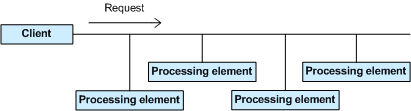
\includegraphics[width=0.6\textwidth]{../images/implementation/embedded_server/demo-chain-of-responsibility-1.png}
	\caption{The idea of  Chain of Responsibility software design pattern}
	\label{fig:chain_of_responsibility}
 \end{figure}
\end{center}
The idea of this pattern is that client request is processed by a chain of processing units.
Each processing unit takes request from previous chain member, makes processing and gives processed object to the next chain member.
This chain can be easily changed by adding or removing processing units and replacing their position in the chain.

The reader needs to create a new packet, assign type
\texttt{PKG\_TYPE\_OUTGOING\_MESSAGE\_STRING}, assign payload (
\texttt{strbuffer\_t} is a simple character buffer structure) and to put this
packet to \texttt{dataInputQueue} from the task configuration.

UART writer pulls the same structured packet from the response queue, checks
that packet type is \texttt{PKG\_TYPE\_OUTGOING\_MESSAGE\_STRING}, extracts the
payload and sends the data back to the client. It is also responsible of
cleaning the memory, it needs to destroy this packet ( by calling appropriate
method)

Reader gives the work to message parser task.
This embedded server implementation uses 
JSON data structures and JSON-RPC protocol  as primary  message passing technology.
They were covered before and some client-server communication was introduced (see listing \ref{lst:jsonrpc_example}). 
The message parser task takes string messages from message queue and converts them into JSON request objects. 
It receives system packet with a type \texttt{PKG\_TYPE\_INCOME\_MESSAGE\_STRING} and makes a \texttt{PKG\_TYPE\_INCOME\_JSONRPC\_REQUEST}  from it.
Parsed JSON-RPC requests are added to the request queue by this task.

JSON website \cite{json_org} contains an overview of available JSON serialization and deserialization libraries.
I have tried some of them, which claimed to be very lightweight: Jansson
(\url{http://www.digip.org/jansson/}), parson
(\url{http://kgabis.github.io/parson/}) and jsmn
(\url{http://zserge.bitbucket.org/jsmn.html}).
I was also tried to write my own
JSON parser, but after some progress i realized, that i am writing something similar to those ready libraries.
I decided to take one of them and to use in my project.

The last one, jsmn JSON parser library, is the most lightweight solution i have ever seen.
It suits well for the embedded systems without dynamic  memory allocation. 
This is a stream based parser and it does not hold copied of data, but holds only references to them.
The regular usage includes declaration of static array of token structures. 
A token is a structure that represents JSON object. 
It has a type and pointers to the original character data of character JSON message.
There are no separate copies stored, API provides only pointers to data.
You need to define the array of tokens in the code, that will be enough to process a new message. 
Parser API function returns a status code that can be a success, parsing error or lack of tokens in the token array.
You can process the tokens if there was a success at parsing step.
Some finite state machine needs to be implemented for this. As the result, it requires more complex processing code (like stream based parser do).
It is not convenient to use such API, this library requires a more beautiful wrapper.

The main choice of JSON parsing library consisted of the battle between Jansson and parson.
Jansson was chosen to be used in this project, because of the custom memory allocation and more elegant API.
It also has a very good documentation with examples and explanations.

\begin{listing}[H]
\begin{minted}[frame=lines,
               framesep=2mm]{c++}
json_t *array, *integer;

array = json_array();
integer = json_integer(42);

json_array_append(array, integer);
json_decref(integer); 
\end{minted}
\caption{Examples of using Jansson library API}
\label{lst:jansson_example}
\end{listing}

This library uses the object reference counting for managing the lifecycle of the objects.
The reference count is used to track whether a JSON object is still in use or not. 
When a value is created, it’s reference count is set to 1. 
If a reference to a value is kept (e.g. a value is stored somewhere for later use), its reference count is incremented, and when the value is no longer needed, the reference count is decremented. 
When the reference count drops to zero, there are no references left, and the value can be destroyed and memory is freed.
This gives a possibility to make complex nested object structures and there is no need of tracking each object separately.
Complex objects can be deleted by decrementing the reference count of the root objects. 
Jansson library recursively decrements count of all nested objects and if reference count becomes zero object is destroyed.

Income message parsing task uses Jansson library to parse incoming JSON-RPC requests.
When request object is parsed it is checked for compatibility with JSON-RPC version 2.0(checks for valid JSON object members). 
Request identificator (\texttt{id}) is exctracted from JSON object and assigned to the packet identificator inside parser task.
The \texttt{id} is a positive integer which has \texttt{json\_int\_t} type (this is actually defined as \texttt{unsigned long long} inside Jansson library).
It is more convenient and efficient to store and later use raw id value for the packet, than to extract the \texttt{id} from JSON object every time
( which requires a hash table lookup inside member extract function, which is more expensive than reading a single variable)


The next processing unit in the request chain of responsibility is the request handler task.
This is the main request handling module in this system.
Listing \ref{lst:request_handler_algorithm} contains an algorithm description of request handler task written in C like pseudocode: 

\begin{listing}[H]
\begin{minted}[frame=lines,
               framesep=2mm]{c++}
while(1) {
	if(requestQueueHasRequests()) {
		request = getRequestFromQueue();
		if(request && (typeof(request) == JSONRPC_REQUEST)) {
			response = handleRequest(request);			
		} else {
			reportError();
		}
		destroyRequest(request);
		if(response) {
			sendResponseToResponseQueue(response);
		}		
	}
}
\end{minted}
\caption{Request hadler algorithm}
\label{lst:request_handler_algorithm}
\end{listing}

The request handling method contains a table of available methods and the method name from the request is searched in that table.
If method was found, a function that corresponds to that particular method is called and the request is passed as the parameter to that function.
The method not found error response is returned if there is no such method available.
I have developed several demo methods to demonstrate coffee machine service functionality
\autoref{tbl:service_remote_methods} contains description of available methods in this system.


\begin{longtabu} to \linewidth {|p{3cm}|p{1.5cm}|X|p{7cm}|}
%\hline
%\rowfont\bfseries H1 & H2 & H3 & H4 
%\endhead

% \\ \hline
% \multicolumn8{r}{There is more to come} \\
% \endfoot

% \\ \hline
% \endlastfoot

% \hline \hline
% \endlastfoot

\hline 
\multicolumn{1}{|l|}{\textbf{Method name}} & 
\multicolumn{1}{l|}{\textbf{Input parameters}} &
\multicolumn{1}{l|}{\textbf{Method output}} &  
\multicolumn{1}{l|}{\textbf{Description}} \\ 
\hline 
\endfirsthead

\multicolumn{4}{l}%
{{\bfseries \tablename\ \thetable{} -- continued from previous page}} \\
\hline 
\multicolumn{1}{|l|}{\textbf{Method name}} & 
\multicolumn{1}{l|}{\textbf{Input parameters}} &
\multicolumn{1}{l|}{\textbf{Method output}} &  
\multicolumn{1}{l|}{\textbf{Description}} \\ 
\hline 
\endhead

\hline \multicolumn{4}{|r|}{{Continued on next page}} \\ \hline
\endfoot

% \hline \hline
\endlastfoot


%\begin{longtable}{|p{0.2\texwidth}|p{0.2\texwidth}|p{0.2\texwidth}|p{0.4\texwidth}|}
%\begin{longtable}{| l | l | l | p{5cm} |}
%	\centering	
	%\begin{tabularx}{\textwidth}{|X|X|X|X|}
% 		\hline
% 		\textbf{Method name} &
% 		\textbf{Input parameters}  	&
% 		\textbf{Method output} &
% 		\textbf{Description} &
			
	    
	%    \tabularnewline
	%	\hline
		"system.help" &
		-- &
		Full service description. &
		Service contract is returned by this method. 
		This is a structured JSON document, that contains a  description of available mehtods similar to this table. 
		
		\tabularnewline
		\hline
		"machine.\newline~getInfo" &
		-- &
		Information about coffee machine &
		This method returns to a client a JSON object with name of connected coffee machine and machine firmware version.

		\tabularnewline
		\hline
		"machine.\newline~getProducts" &
		-- &
		List of available products &
		A complete list of available products is returned.
		The members of that list are JSON structures that define a product.
		They contain the name of a product, its code and the price.
		
		\tabularnewline
		\hline
		"machine.\newline~orderProduct" &
		A product code &
		Returns a status of order operation. &
		This method call starts coffee prepearing procedure on the coffee machine.
		Valid product code, that was received as a result from  "machine.getProducts" should be provided.
		Method returns the status of operation which can be one of follows: \newline
		"PRODUCT\_STATUS\_STARTED" \newline
		"PRODUCT\_STATUS\_FAILED" \newline 
		"PRODUCT\_STATUS\_BUSY" 
		The last status is returned if this product is already running.
		
		
		\tabularnewline
		\hline
		"machine.\newline~getProductStatus" &
		A product code &
		Returns a status of previously started product order. &
		This method call is used for retrieving a status of coffee product currently being prepared.
		Valid product code, that was received as a result from  "machine.getProducts" should be provided.
		Method returns the status of operation which can be one of follows: \newline
		"PRODUCT\_STATUS\_STARTED" \newline  
		"PRODUCT\_STATUS\_IN\_PROGRESS" \newline 
		"PRODUCT\_STATUS\_FINISHED" \newline 
		"PRODUCT\_STATUS\_FAILED" 
		
		\tabularnewline
		\hline
		"machine.\newline~cancelProduct" &
		A product code &
		Returns a status of cancel operation &
		Possible values are: \newline
		"PRODUCT\_STATUS\_CANCELLED" \newline 
		"PRODUCT\_STATUS\_FAILED"
		
		
		\tabularnewline
		\hline
	%\end{tabularx} 
	\caption{Embedded service remote methods}
	\label{tbl:service_remote_methods}
\end{longtabu}




Each handler method receives and returns an JSON-RPC message object. 
Some methods are communicating to a directly connected coffee machine and trigger some events there.
This communication is using closed proprietary protocol and these methods are working with a special library from the manufacturer.
This library was provided to me and was partially implemented by me.
User code need only to execute a methods from that library and receive a result.
Library internals write requests to the coffee machine and receiving response messages using UART transciever.
Library specification is the C language header file, where are defined all function prototypes and return codes. 
The coffee machine manufacturer insisted of not publishing the details of protocol used and the implementation of that library.
We are using it here in the design with the assumption, that it does its communication work well, with any knowledge of internal behaviour of that software module (black box).
This was one of the main reasons why a proxy/translator architecture ( mentioned here \ref{sec:device_connection_scheme}) may be used to integrate proprietary and legacy devices into other systems.

Returned response JSON-RPC messages are serialized back to string character data in the request handler task and are inserted to a response queue, where they could be picked by a UART writer task for further writing
(see \autoref{fig:server_components_and_data_flow}).
The last UART writer task writes data to the client interface UART and totally destroys that response message.

Now we have described the whole data flow cycle of this system architecture.
One of the main design goals it that system packets are created and deleted only once inside Reader and Writer software modules near the corresponding client interface.
Other processing units are only changing the internal packet structure by changing packet type and payload of the packet.
This reduces overall memory consumption.

The architecture design that is based on queues and separate processing tasks help to produce an extensible and scalable systems.
When some task becomes a throughput bottleneck there is always an opportunity to add the another same task in parallel. 
Two or more tasks can receive the work from one queue and more than one task could push the results into one destination queue.
Processing units in between can be changed or totally replaced, because input and output interface of the modules is defined.
For example, if we decide to change the netstrings message encoding for something else, we  only need to rewrite Reader and Writer modules.
JSON to XML data serialization replacement requires more fundamental changes (because JSON object is used as primary data transfer objects in the request handle methods, therefore you need to rewrite all request methods to solve that problem), but if the underlying communication transport structure is not changed, it is not necessary to touch this part of the system.


\subsubsection{Service description contract}
\label{sec:service_json_contract}

As you already know, the whole system i based on the JSON-RPC specification.
Service description contract is also made using similar technologies.
\autoref{sec:appendix_service_contracts} provides an examples of service contracts.
JSON version of contract is inspired from JSON Schema Service Descriptor Draft at \url{http://www.simple-is-better.org/}.
There is a specification of service interface description, which is similar to the \gls{WSDL} from WS-* technologies. 
Service contract of coffee machine service is made according to that specification.

It uses a JSON-Schema\footnote{\url{http://json-schema.org/}} specification to describe the JSON data format. 
JSON object could also be self desctiptive and automatically verified by the machine.
There is no official standard available yet, but most of these technologies are in the development phase right now. 
These are mostly working drafts.
JSON-Schema is supported by the IETF(Internet Engineering Task Forse) organization and there is a big hope that these JSON technologies become an production standard.


\begin{listing}[h]
\begin{minted}[frame=lines,
               framesep=2mm]{json}
{
    "description": "A geographical coordinate",
    "type": "object",
    "properties": {
        "latitude": { "type": "number" },
        "longitude": { "type": "number" }
    }
}
\end{minted}
\caption{JSON-Schema definition of geographic coordinate object}
\label{lst:json_schema_geo}
\end{listing}

JSON is a great and more lightweight alternative for XML.
Web Services and related XML technologies become a de facto standard for large corporate service systems. 
There are developed by large corporations like Microsoft, IBM, Oracle who have personal interest of these technologies.
These standards are more bureaucratic that simple and verbose JSON solutions. 

Author of this work tries to say that service oriented technologies can be implemented not only using XML, SOAP and HTTP.
There are lots of other alternatives and the implementation of correct solution
depends on the target application.
I needed more compact and lightweight protocol, because of the target hardware. 

\hyperref[lst:json_contract_example]{Provided} 
JSON service descriptor contains the declaration of implemented methods and their input parameters structures and types of returned objects.
Service contract can be received as a response of "system.help" method
The communication could look like:

\begin{listing}[H]
\begin{minted}[frame=lines,
               framesep=2mm]{javascript}
-->  {"jsonrpc": "2.0", "method": "system.help", "id": 1}
<--  {"jsonrpc": "2.0", "result": { Service contract object here}, "id": 1}
\end{minted}
\caption{Acquisition of service contract}
\label{lst:service_contract_acquisition}
\end{listing}

There could be also any defined character sequence that tells the server to response with the documentation object.
Imagine that you are connecting to an old legacy device using serial line communication.
You have found it in your basement within the old gadgets of your  grandfather. 
You connect some wires, open a serial terminal and do not know what to do next.
There is no protocol description nearby and the internet has only few unclear reference to the text written on the device box.
You start typing some chaotic text in the terminal and  send it to the device, and device does not respond you.
After some retries are made, you receive a huge text containing the specification of this device.
For example, server may respond to some of received character sequences:
\begin{listing}[H]
\begin{minted}[frame=lines,
               framesep=2mm]{javascript}
-h
--help
{"jsonrpc": "2.0", "method": "system.help", "id": 1}
"^*[Hh][Ee][Ll][Pp]*$" regular expression values
... to be continued
\end{minted}
\caption{Server may return service contract description after he receives these characters from communication line}
\label{lst:server_help_return}
\end{listing}


PROFIT! Now you could game with the recovered device.

Service contract provide an easy and descriptive way how to search for available piece of functionality.
You can call remote procedures right after you have received this kind of specification. 

%  One solution is to use closed encrypted proprietary
% protocol and be calm, but as it was mentioned earlier, it limits the possibility of integration
% between other embedded systems. It this case all of your devices should support
% that protocol and you choise of different hardware is limited. Proprietary
% protocols are often vendor-specific, code is closed, documentation is not free
% and all it works only with the proprietary devices from the manufacturer.
% 
% 
% \begin{center}
%  \begin{figure}[h]
% 	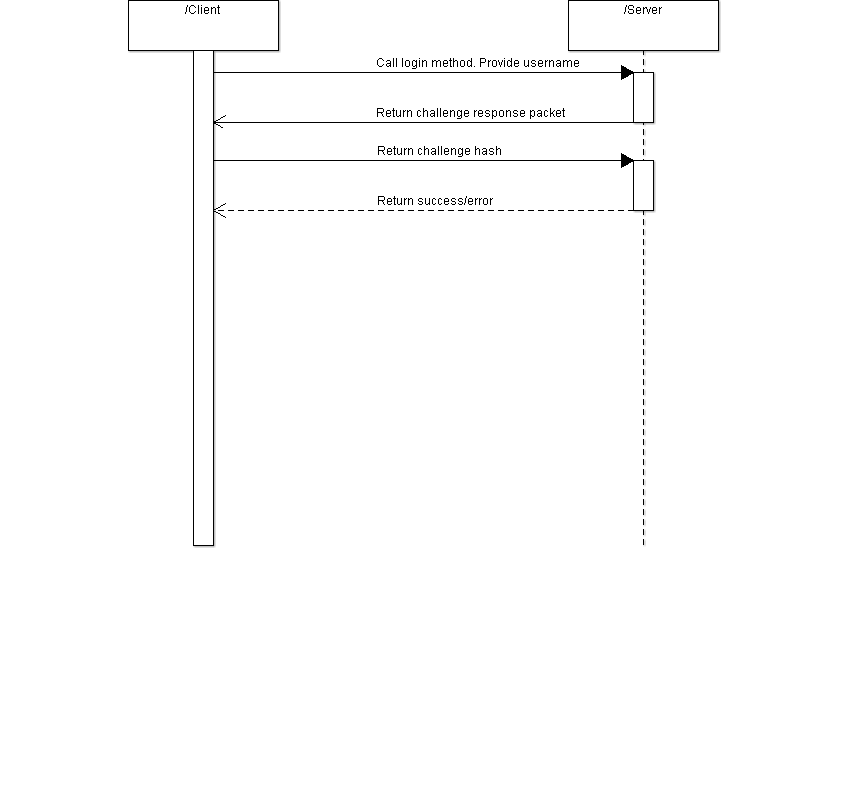
\includegraphics[width=\textwidth]{../images/implementation/embedded_server/SequenceDiagram.png}
% 	\caption{Client authentification process}
% 	\label{fig:embedded_server_login_auth}
%  \end{figure}
% \end{center}

%reversably encrypted form.

